%
% hardware.tex
%
% Copyright (C) 2019 by Universidade Federal de Santa Catarina.
%
% OBDH 2.0 Documentation
%
% This work is licensed under the Creative Commons Attribution-ShareAlike 4.0
% International License. To view a copy of this license,
% visit http://creativecommons.org/licenses/by-sa/4.0/.
%

%
% \brief Hardware chapter.
%
% \author Gabriel Mariano Marcelino <gabriel.mm8@gmail.com>
%
% \institution Universidade Federal de Santa Catarina (UFSC)
%
% \version 0.1.0
%
% \date 20/10/2019
%

\chapter{Hardware} \label{ch:hardware}

\section{Interfaces}

\begin{figure}[!ht]
    \begin{center}
        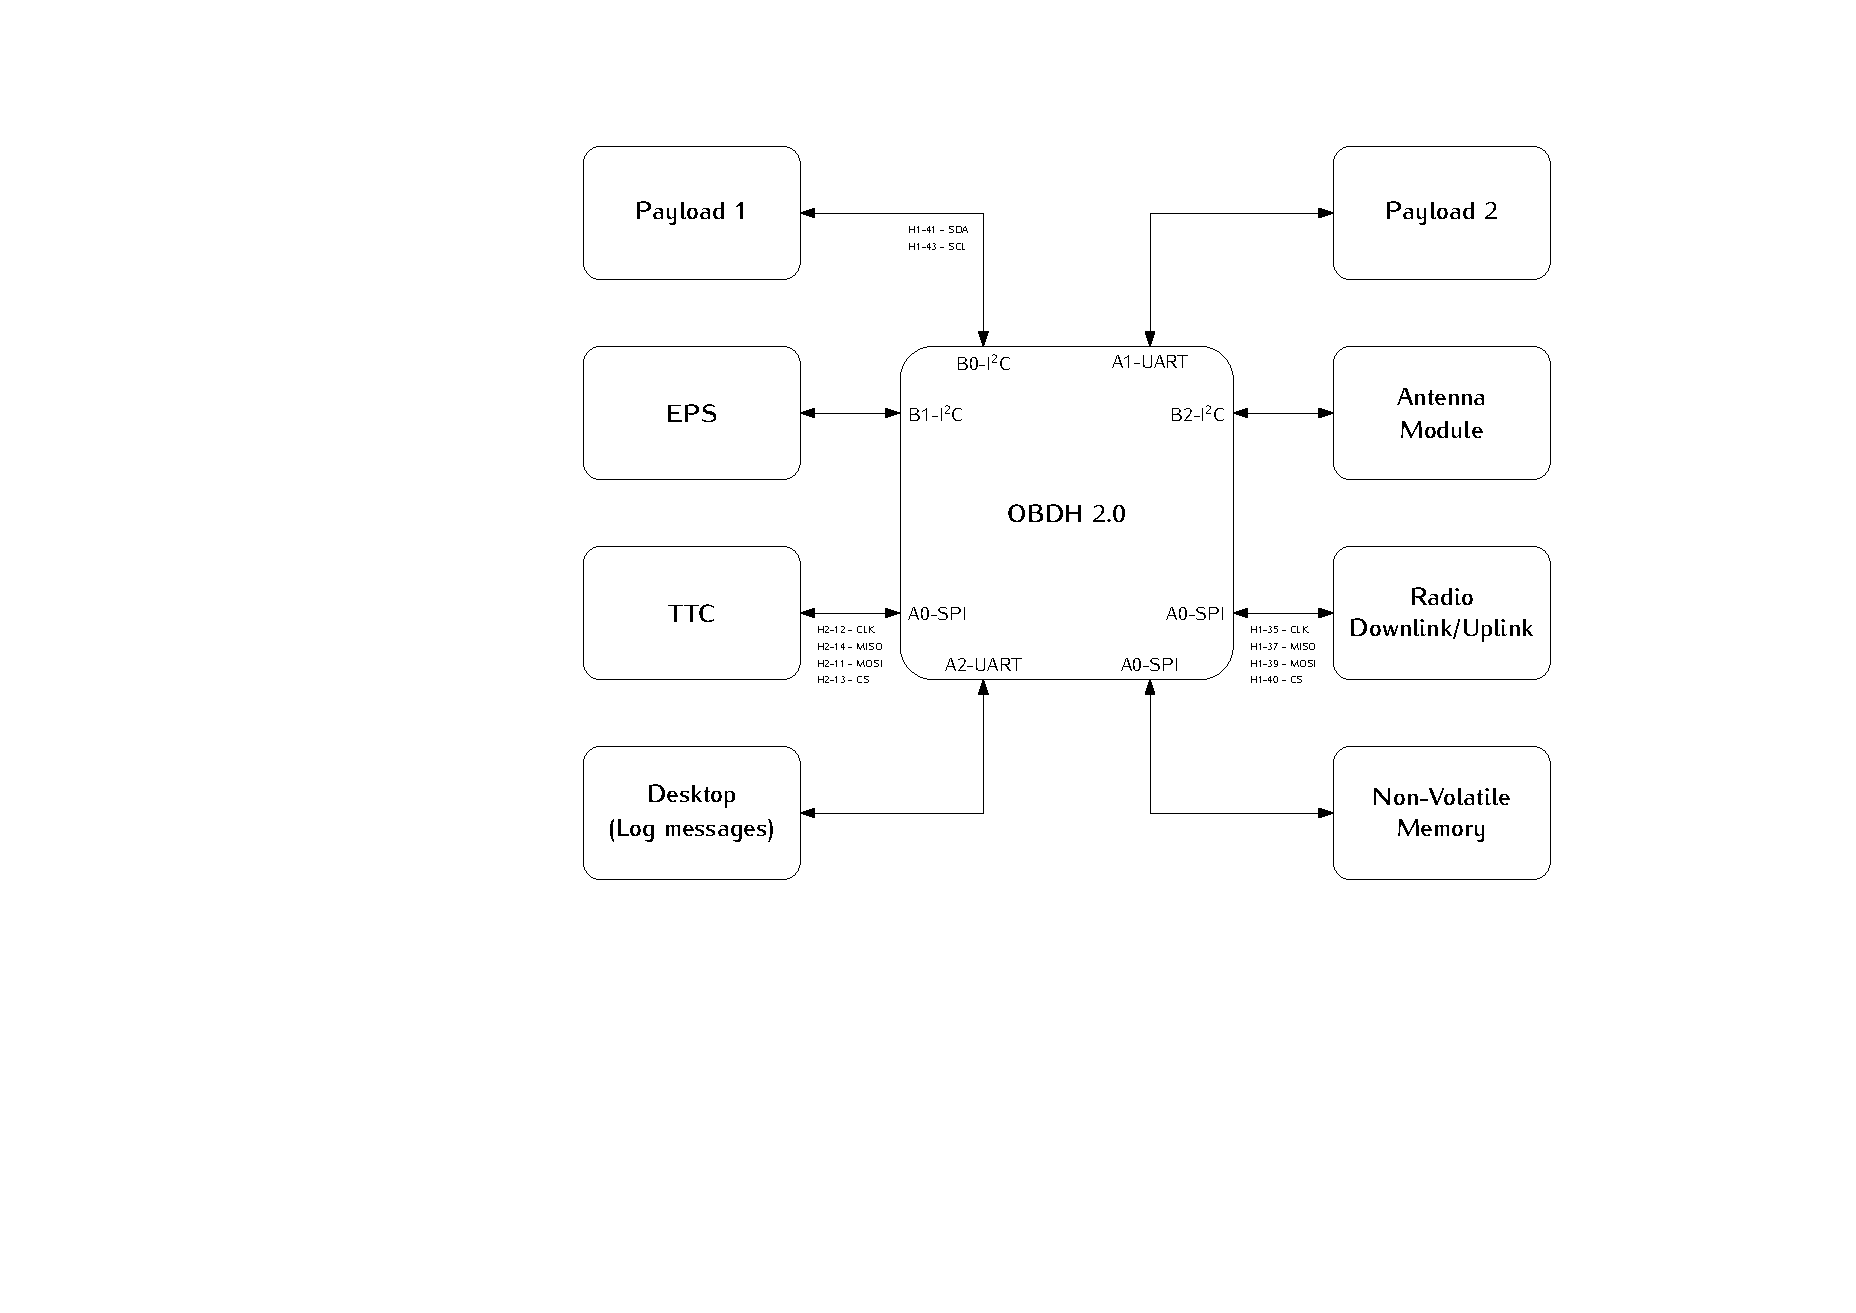
\includegraphics[width=\textwidth]{figures/diagram_interfaces.pdf}
        \caption{Interfaces diagram.}
        \label{fig:diagram-interfaces}
    \end{center}
\end{figure}

Currently, ``\textit{Payload 1}'' and ``\textit{Payload 2}'' are ``\textit{Payload-X}'' and ``\textit{Payload EDC}'' respectively.

\section{External Connectors}

\subsection{PC-104}

\begin{table}[!h]
    \centering
    \begin{tabular}{cllll}
        \toprule[1.5pt]
        \textit{Pin [A-B]} & \textit{H1A}     & \textit{H1B}     & \textit{H2A}  & \textit{H2B}  \\
        \midrule
        1-2                & -                & -                & -             & -             \\
        3-4                & -                & -                & -             & -             \\
        5-6                & GPIO\_0          & GPIO\_1          & -             & -             \\
        7-8                & GPIO\_2          & GPIO\_3          & -             & -             \\
        9-10               & GPIO\_4          & -                & -             & -             \\
        11-12              & GPIO\_5          & GPIO\_6          & SPI\_0\_MOSI  & SPI\_0\_CLK   \\
        13-14              & GPIO\_7          & -                & SPI\_0\_CS\_1 & SPI\_0\_MISO  \\
        15-16              & -                & -                & -             & -             \\
        17-18              & -                & GPIO\_8          & -             & -             \\
        19-20              & -                & GPIO\_9          & -             & -             \\
        21-22              & -                & -                & -             & -             \\
        23-24              & -                & -                & -             & -             \\
        25-26              & RS485\_TX+       & RS485\_TX-       & -             & -             \\
        27-28              & RS485\_RX+       & RS485\_RX-       & -             & -             \\
        29-30              & GND              & GND              & GND           & GND           \\
        31-32              & GND              & GND              & GND           & GND           \\
        33-34              & -                & -                & -             & -             \\
        35-36              & SPI\_0\_CLK      & -                & VCC\_3V3\_ANT & VCC\_3V3\_ANT \\
        37-38              & SPI\_0\_MISO     & -                & -             & -             \\
        39-40              & SPI\_0\_MOSI     & SPI\_0\_CS\_0    & -             & -             \\
        41-42              & I2C\_0\_SDA      & -                & -             & -             \\
        43-44              & I2C\_0\_SCL      & -                & -             & -             \\
        45-46              & VCC\_3V3         & VCC\_3V3         & -             & -             \\
        47-48              & -                & -                & -             & -             \\
        49-50              & -                & -                & -             & -             \\
        51-52              & -                & -                & -             & -             \\
        \bottomrule[1.5pt]
    \end{tabular}
    \caption{PC-104 connector pinout.}
    \label{tab:pc104-pins}
\end{table}

\subsection{Antenna Module}



\subsection{Programmer}



\subsection{Debug Interface}



\subsection{Daughter Board}



\section{Microcontroller}

MSP430F6659.

\section{Non-Volatile Memory}

The non-volatile memory is composed by a NOR flash memory with 1 Gb of capacity (or 128 MB). The used model is the Micron MT25QL01GBBB.

As can be seen in \autoref{fig:diagram-interfaces}, a SPI bus is used to communicate with this peripheral.
